This chapter describes briefly the origins and motivations that lead to the collection and curation of the data used in this thesis, as well as some of its main features.


\section{The CompMusic Project}\label{compmsc}

The mp3 files and labels comprising the carnatic corpus that was used in this thesis were gathered as part of the {\it CompMusic: Computational Models for the discovery of the world's music} project, promoted by Professor Xavier Serra at the Universitat Pompeu Fabra (Barcelona) since 2011 and funded by the European Research Council. As described by Professor Serra himself\cite{serra-comp14}, ``The focus of the project lies on computational approaches to describe music recordings by emphasising the use of domain knowledge of particular music traditions, focusing on five music cultures: Arab-Andalusian (Maghreb), Beijing Opera (China), Turkish-makam (Turkey), Hindustani (North-India) and Carnatic (South-India)''. This can be encompassed within the scientific field of Music Information Research (MIR), which ``primarily addresses topics involved in the understanding and modeling of music using information processing methodologies. In particular, it aims to advance our knowledge in representing, understanding, describing, retrieving, archiving and organizing music related data''\cite[p.3]{gulati}.\\

Specifically, CompMusic aims to help overcoming the information bias towards western music present in the MIR field, in order to achieve a broader and more profound understanding of different culture-specific musical phenomena, as well as develope domain-specific research methodologies more appropiate to solve them. Part of the underlying thesis is that ``addressing the research problems in the context of diverse music cultures will not only help in advancing the knowledge in the specific cultures, but also expand the scope of the state of the art in MIR''\cite[p.4]{gulati}. Further quoting, ``Among ethnomusicologists there is a wide consensus that all musics are not alike, and that the approaches used to understand Western musics are not appropriate for other types of musics.''\cite{serra-comp14}. A further and very detailled explanation on the motivations and implications of the project can be found in \cite{serra-comp11} and \cite{serra-comp14}.\\

The creation and curation of the diferent corpora in the context of the CompMusic project responds to a double motivation: it allows the reproducibility of the experiments, and also serves as basis for any data-driven approach that may also be undertaken. For that sake, the CompMusic project has developed the Dunya platform, ``a tool for navigating through music collections which also acts as the central permanent online repository to store the metadata, audio, annotations and research results. Dunya is open source and provides an API for accessing these data''\cite{indian-corpora}.\\

Prof. Serra's research group kindly granted us access to the platform's contents via its open API (\url{https://github.com/MTG/dunya}), and, for the carnatic corpus, we were able to download a total of 2455 labeled recordings as high-quality mp3 files of different lengths. The labels comprise ten different domains: \texttt{r\=aga}, \texttt{form}, \texttt{title}, \texttt{work}, \texttt{album\_artists}, \texttt{t\=a\d{l}a}, \texttt{length}, \texttt{artists}, \texttt{mbid} and \texttt{concert}. The histograms of total length and number of recordings per class can be found in appendix \ref{ds-stats}, for all domains except \texttt{length}, \texttt{title} and \texttt{work} (since they would have one class per sample and such histograms wouldn't be meaningful). Bear in mind that, in some domains, a single recording may appear in several classes (for instance, an ensemble has always several \texttt{album\_artists}), and, for some recordings, several domains may remain unlabeled hence not appearing in all the histograms. Therefore, the overall distribution is different for each domain. The 2014 article cited in \cite{indian-corpora} contains some further statistics, but the corpus has changed considerably since then, as it can be seen in the data presented here (for example, now it has over 500 more recordings, but 25 less r\=agas). In any case, the article contains also further useful information about the agents involved in the compilation and labelling process of all CompMusic's corpora, which may be interesting for curation purposes but outside of the scope of this thesis.\\

For a more detailled description of the dataset's musical contents, see chapter \ref{about-car}.


\section{The R\=aga Recognition Dataset (\(RRD_{CMD}\))} \label{rrd_cmd}

A relevant subset of the carnatic corpus in the context of this thesis is the (\(RRD_{CMD}\)) dataset, introduced by Gulati et al. in 2016 (see \cite[p.84]{gulati}). As a part of the CompMusic project, \(RRD_{CMD}\) was selected and curated to provide a sizable, fixed subset that would fullfill the above mentioned criteria of purpose, coverage, completeness, quality and reusability (as stated in \cite[pages 7, 10 and 83]{gulati}: see chapter \ref{about-car} for more details on the different r\=agas and their musical aspects).  Its main features are pictured in Figures \ref{fig:rrd-overall} and \ref{fig:rrd-ragasvaras}.\\

As explained in \cite[p.61]{gulati}, this test dataset responds to the idea of a static collection (as opposed to a research corpus which can evolve over time) that allows benchmarking and reproducibility of the research results. More specifically, it notes that it ``should not be confused with the training and testing split of a dataset, which are the terms used in the context of a cross validation experimental setup''. For an explanation about this ``cross validation experimental setup'', see \cite[p.121]{goodfellow}.\\

The dataset features are open and accessible in GitHub: \url{https://github.com/sankalpg/MelodicAnalysisDatasets/tree/master/RagaDataset/Carnatic}.\\
From its 480 listed recordings, only 439 were present in the Dunya platform at the moment of downloading. This remaining subset, noted as \(RRD^*\) from now on, is therefore smaller, but still similarly distributed, as it can be seen in Table \ref{fig:rrd-stats}.

\begin{figure}[h]
  \centering
  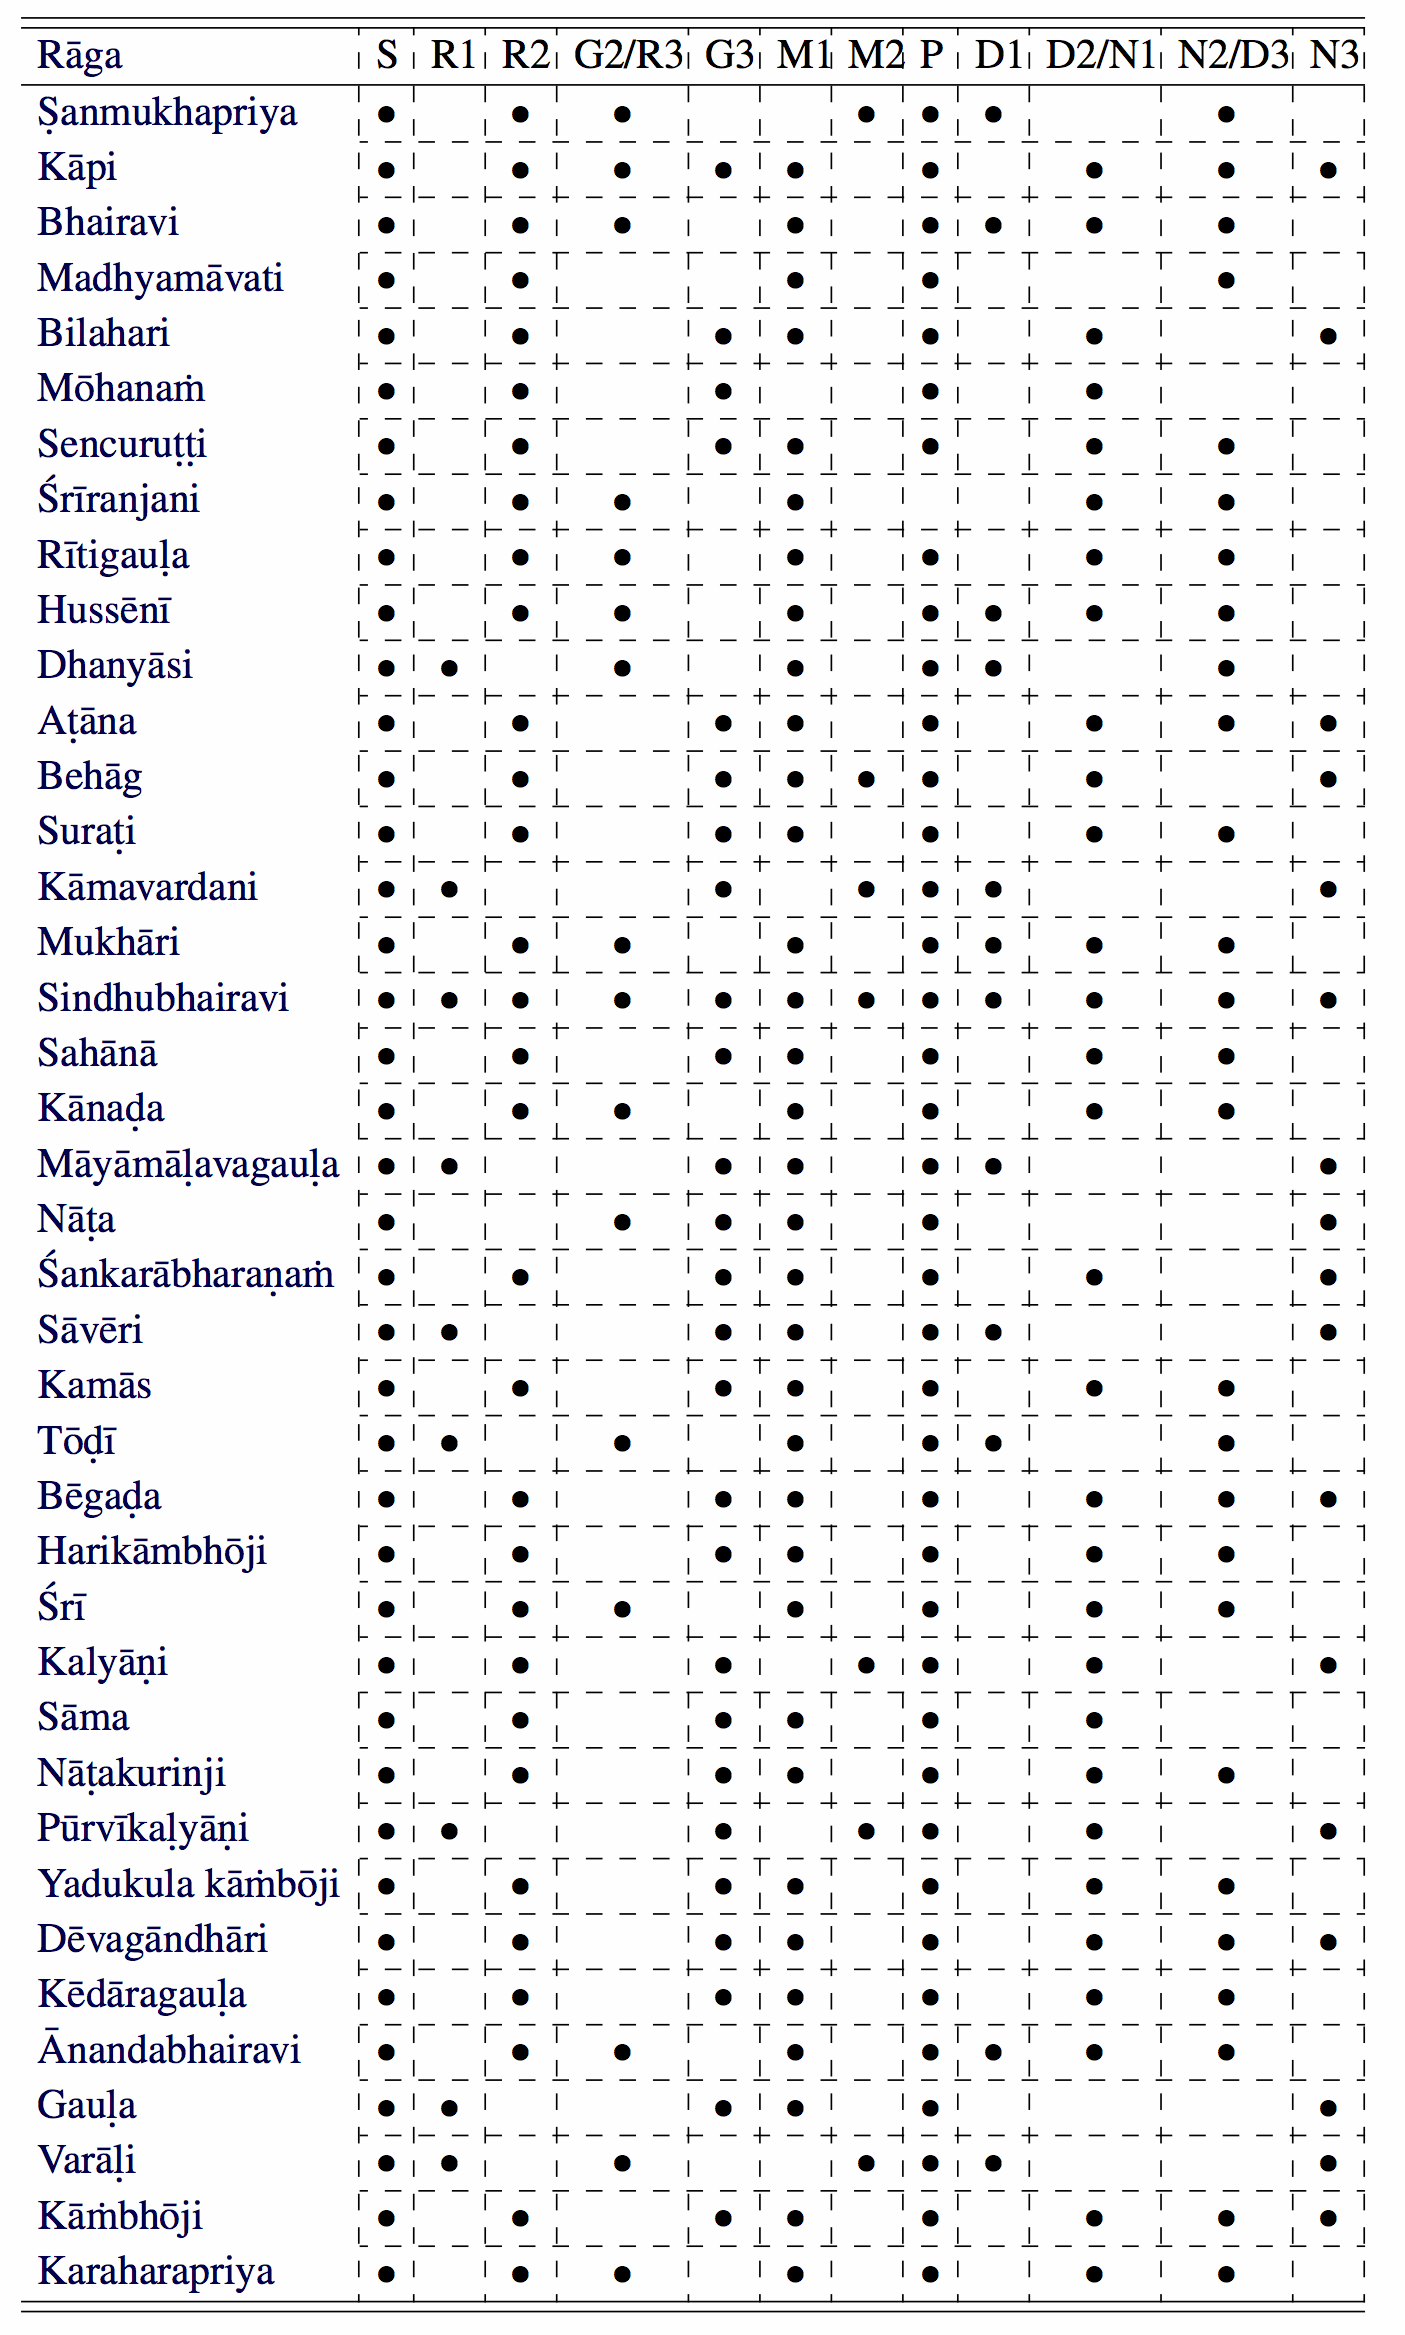
\includegraphics[scale=0.28]{raga_svaras.png}
  \caption{List of the r\=agas in (\(RRD_{CMD}\)) along with their constituent set of svaras. The contents of this table are verified by Vignesh Ishwar, a professional vocalist of carnatic music (from \cite[p.244]{gulati}. See chapter \ref{about-car} of the present thesis for a more detailled description of the r\=agas).}
  \label{fig:rrd-ragasvaras}
\end{figure}

\begin{figure}[h]
  \centering
  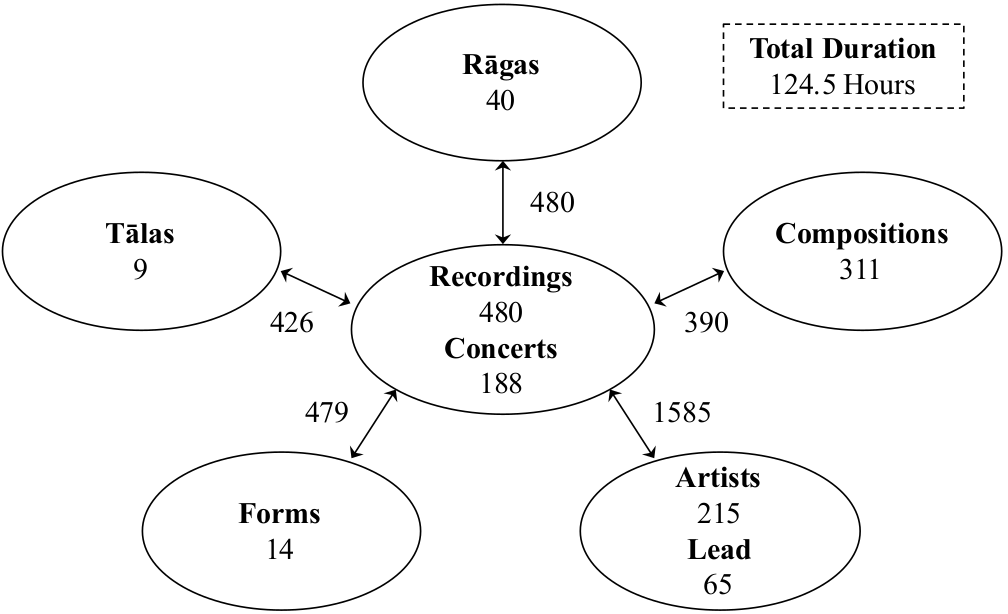
\includegraphics[scale=0.4]{rrd_gulati.png}
  \caption{Details of the rāga recognition dataset (\(RRD_{CMD}\)) comprising Carnatic music recordings in terms of the number of different musical entities and relationships between them. (from \cite[p.85]{gulati}).}
  \label{fig:rrd-overall}
\end{figure}
